
\section{Resultados}

\subsection{Red de interacción entre genes}

Se identificaron un total de 51 genes asociados al fenotipo \textbf{Papilloma} y obtuvimos una representación visual de la red de interacción entre los genes.
\begin{figure}
	\centering
	\includegraphics[width=0.8\linewidth]{figures/cluster_etiq_louvain}
	\caption{Red formada por los 51 genes relacionados con el fenotipo \textbf{Papilloma}}
	\label{fig:grado_centralidad}
\end{figure}

\subsection{Análisis de enriquecimiento funcional}

Se realizó un análisis de enriquecimiento funcional destacando las categorías \textbf{Process} y \textbf{KEGG}, obteniendo relaciones entre algunos grupos de genes con problemas del sistema inmune, carcinoma y las adipoquinas.

Los términos y categorías relacionados con enfermedades como \textbf{cervix}, \textbf{ovarian}, \textbf{HPV}, \textbf{herpes}, \textbf{papillomavirus}, \textbf{costellos} y \textbf{cowden} fueron encontrados en el análisis de enriquecimiento funcional, indicando posibles vínculos entre estos términos y los genes asociados al fenotipo estudiado.

Se realizaron búsquedas específicas de genes clave como \textbf{TP53}, \textbf{AKT1}, \textbf{SDHB}, \textbf{SDHD}, \textbf{HRAS} dentro de las categorías significativas. Estos genes podrían tener una importancia particular en relación con el fenotipo de interés, evidenciando su posible relevancia funcional.

\subsection{Descarga y procesamiento de la red de interacción}

Se descargó la red de interacción en formato TSV. El archivo descargado se procesó para dar como resultado un archivo de texto \textbf{$genes_igraph.txt$} formado por dos columnas de nombres de genes, en las que cada fila representa una relación entre dos genes.



\subsection{Propiedades de la red y detección de comunidades}

En nuestra red vimos que todos los nodos estaban conectados entre sí y que se trataba de un grafo no dirigido.

\vspace{3pt}

Obtuvimos una tabla con el \textbf{grado de centralidad} de cada gen. Pudimos observar como el gen de interés TP53 es el que presentaba un mayor grado de centralidad y por tanto más relaciones con otros genes. 
\begin{figure}
	\centering
	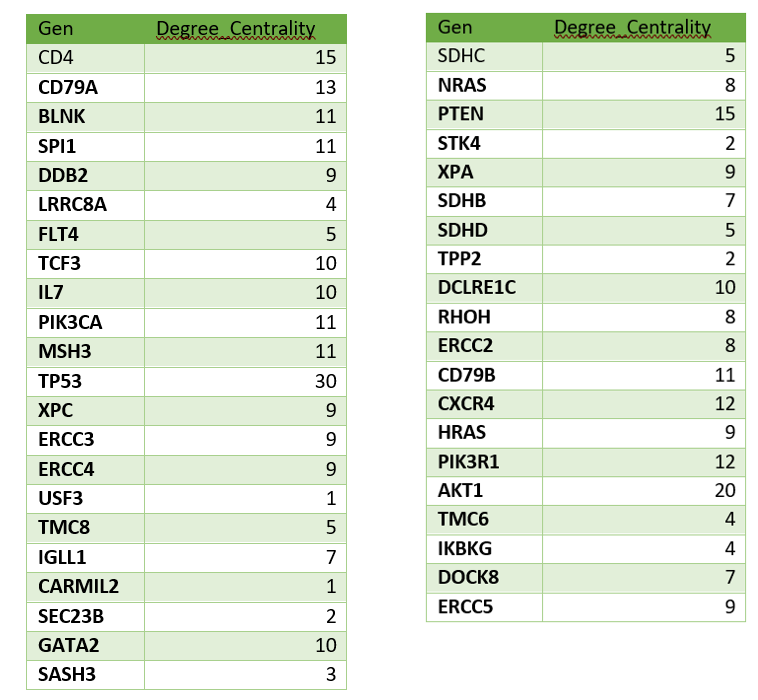
\includegraphics[width=0.8\linewidth]{figures/grado_centralidad}
	\caption{Descripción de la figura.}
	\label{fig:grado_centralidad}
\end{figure}


\vspace{3pt}

En cuanto al \textbf{grado de conectividad} obtuvimos un valor del 19\%, el cual era bastante pequeño y nos indicaba que nuestro grafo no era muy fuerte. Esto puede deberse a que las comunidades entre si no tenían una gran dependencia y teníamos varios genes que no nos interesaban. 

\vspace{3pt}

Empleamos distintos algoritmos para \textbf{detectar comunidades}. En el caso del método de Girvan-Newman había nodos que no pertenecían a ninguna comunidad. Esto podía deberse a la forma en que el algoritmo de betweenness identifica comunidades. Puede detectar comunidades basándose en la centralidad de intermediación de los nodos, y algunos nodos pueden no estar claramente vinculados a una comunidad en función de esta medida.

\vspace{3pt}

Con el algoritmo voraz todos los nodos pertenecían a alguna comunidad. al igual que con el algoritmo de propagación de etiquetas. Sin embargo, en este último obtuvimos tan solo 3 comunidades por lo que la clusterización es mínima.  Con la aplicación del método de Louvain también resultaban menos comunidades que con el algoritmo voraz. Observamos 4 comunidades. 

\begin{figure}
	\centering
	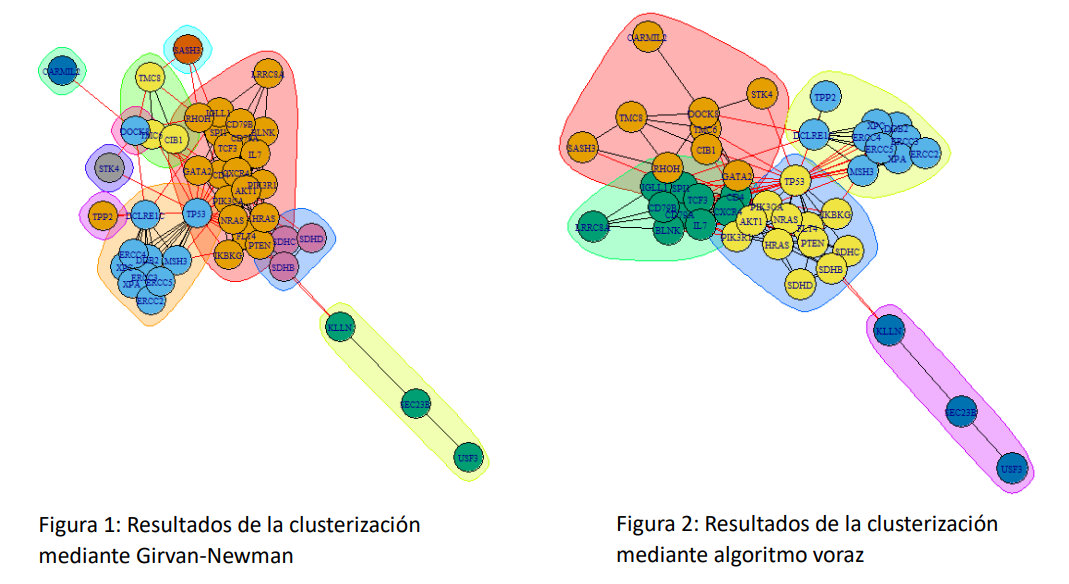
\includegraphics[width=0.8\linewidth]{cluster_GN_voraz}
	\caption{Descripción de la figura.}
	\label{fig:cluster_GN_voraz}
\end{figure} 

\begin{figure}
	\centering
	\includegraphics[width=0.8\linewidth]{cluster_etiq_louvain}
	\caption{Descripción de la figura.}
	\label{fig:cluster_etiq_louvain}
\end{figure}

Los algoritmos anteriores tenían la desventaja de que no reflejaban con exactitud la posibilidad de que un gen perteneciera a más de una comunidad. Para estudiar esto hicimos uso de \textbf{Link Communities}, y obtuvimos una gráfica donde cada gen era representado por un diagrama de sectores. Observamos que la mayoría de los genes pertenecen a más de una comunidad. Al centrarnos en nuestros genes de interés detectamos que el gen \textbf{TP53} tenía relación con 4 clusters distintos mientras que los otros genes de interés, SDHB, SDHb,HRAS, AKT1 se encontraban en una comunidad más diferenciada de color rosa. 

\begin{figure}
	\centering
	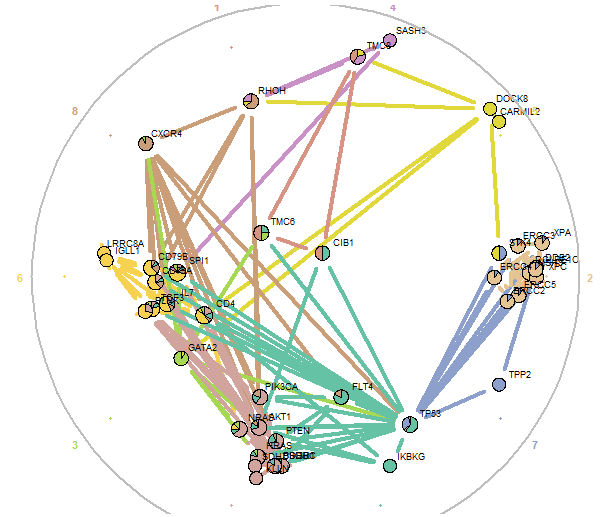
\includegraphics[width=0.8\linewidth]{link}
	\caption{Descripción de la figura.}
	\label{fig:link}
\end{figure}



Para el \textbf{estudio genes de interés} obtuvimos una tabla con dos columnas, el gen en concreto y sus genes vecinos. Observamos que todos los genes estaban relacionados entre sí menos el caso de TP53 y SDHD. 

\begin{figure}
	\centering
	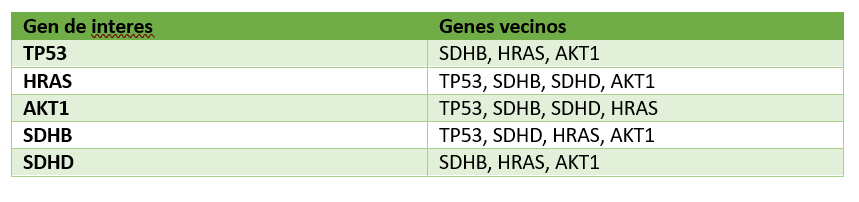
\includegraphics[width=0.8\linewidth]{gen_interes}
	\caption{Descripción de la figura.}
	\label{fig:gen_interes}
\end{figure}

\subsection{Relación de los genes de interés con fenotipos patológicos.}

Tras enriquecer el conjunto de genes de interés hemos obtenido 729 entradas en las cuales hemos encontrado relaciones de genes con fenotipos patológicos como estos:

\begin{table}[h]
	\centering
	\caption{Fenotipos patológicos con palabra clave papiloma}
	\begin{tabular}{|c|c|}
		\hline
		\textbf{Genes} & \textbf{Fenotipos patológicos asociados} \\
		\hline
		FLT4,PIK3CA,TP53,SDHC,NRAS,PTEN,SDHB,SDHD,HRAS,PIK3R1,AKT1,IKBKG & Papiloma \\
		\hline
		TP53,NRAS & Papiloma del plexo coroideo \\
		\hline
	\end{tabular}
\end{table}

\begin{table}[h]
	\centering
	\caption{Fenotipos patológicos con palabra clave papiloma}
	\begin{tabular}{|c|c|}
		\hline
		\textbf{Genes} & \textbf{Fenotipos patológicos genital} \\
		\hline
		PIK3CA,TP53,SDHC,NRAS,PTEN,SDHB,SDHD,AKT1 & Neoplasia genital \\
		\hline
		FLT4,PIK3CA,TP53,SDHC,NRAS,PTEN,SDHB,SDHD,HRAS,AKT1 & Anomalía de los genitales externos masculinos \\
		\hline
		PIK3CA,TP53,SDHC,NRAS,PTEN,SDHB,SDHD,AKT1 & Morfología anormal de los genitales internos femeninos \\
		\hline
	\end{tabular}
\end{table}

\begin{table}[h]
	\centering
	\caption{Fenotipos patológicos con palabra clave renal}
	\begin{tabular}{|c|c|}
		\hline
		\textbf{Genes} & \textbf{Fenotipos patológicos asociados} \\
		\hline
		PIK3CA,TP53,SDHC,NRAS,PTEN,SDHB,SDHD,AKT1 & Neoplasia renal \\
		\hline
		PIK3CA,SDHC,NRAS,PTEN,SDHB,SDHD,AKT1 & Carcinoma de células renales \\
		\hline
		PIK3CA,TP53,SDHC,PTEN,SDHB,SDHD,AKT1 & Anomalía de las glándulas suprarrenales \\
		\hline
		TP53,SDHC,PTEN,SDHB,SDHD & Neoplasia de la glándula suprarrenal \\
		\hline
		SDHC,SDHB,SDHD & Feocromocitoma extraadrenal \\
		\hline
		SDHC,SDHB,SDHD & Feocromocitoma suprarrenal \\
		\hline
	\end{tabular}
\end{table}

\begin{table}[h]
	\centering
	\caption{Fenotipos patológicos con palabra clave carcinoma}
	\begin{tabular}{|p{3cm}|p{4cm}|}
		\hline
		\textbf{Genes} & \textbf{Fenotipos patológicos asociados} \\
		\hline
		PIK3CA, SDHC, NRAS, PTEN, SDHB, SDHD, HRAS, AKT1 & Carcinoma folicular de tiroides \\
		\hline
		PIK3CA, TP53, SDHC, NRAS, PTEN, SDHB, SDHD, HRAS, AKT1 & Carcinoma de tiroides \\
		\hline
		PIK3CA,TP53,SDHC,PTEN,SDHB,SDHD,AKT1 & Carcinoma de mama \\
		\hline
		PIK3CA,SDHC,NRAS,PTEN,SDHB,SDHD,AKT1 & Carcinoma de células renales \\
		\hline
		PIK3CA,SDHC,PTEN,SDHB,SDHD,AKT1 & Carcinoma de endometrio \\
		\hline
		PIK3CA,NRAS,PTEN,HRAS,AKT1 & Carcinoma de células transicionales de vejiga \\
		\hline
		PIK3CA,NRAS,AKT1 & Carcinoma colorrectal hereditario no polipósico \\
		\hline
		NRAS,HRAS1 & Carcinoma no medular de tiroides \\
		\hline
		PIK3CA,AKT1 & Adenocarcinoma papilar de ovario \\
		\hline
		PIK3CA,TP53 & Adenocarcinoma de pulmón \\
		\hline
		NRAS,HRAS & Carcinoma papilar de tiroides \\
		\hline
		NRAS,HRAS & Carcinoma basocelular \\
		\hline
		PIK3CA,TP53 & Carcinoma hepatocelular \\
		\hline
		TP53,AKT1 & Carcinoma \\
		\hline
	\end{tabular}
\end{table}

\begin{table}[h]
	\centering
	\caption{Fenotipos patológicos con palabra clave ovario y derivados}
	\begin{tabular}{|c|c|}
		\hline
		\textbf{Genes} & \textbf{Fenotipos patológicos asociados} \\
		\hline
		PIK3CA,TP53,PTEN,AKT1 & Neoplasia ovárica \\
		\hline
		PIK3CA,AKT1 & Adenocarcinoma papilar de ovario \\
		\hline
		PIK3CA,TP53,SDHC,PTEN,SDHB,SDHD,AKT1 & Anomalía del ovario \\
		\hline
		PIK3CA,SDHC,PTEN,SDHB,SDHD,AKT1 & Ovarios poliquísticos agrandados \\
		\hline
	\end{tabular}
\end{table}

\begin{table}[h]
	\centering
	\caption{Fenotipos patológicos con palabra clave útero y derivados}
	\begin{tabular}{|c|c|}
		\hline
		\textbf{Genes} & \textbf{Fenotipos patológicos asociados} \\
		\hline
		PIK3CA,SDHC,NRAS,PTEN,SDHB,SDHD,AKT1 & Neoplasia uterina \\
		\hline
		PIK3CA,NRAS,AKT1 & Leiomiosarcoma uterino \\
		\hline
		FLT4,SDHB,SDHD,PIK3R1 & Retraso del crecimiento intrauterino \\
		\hline
	\end{tabular}
\end{table}
\clearpage
